\documentclass{article}

 % https://tex.stackexchange.com/a/80510/71579
\usepackage[paperheight=20cm,paperwidth=40cm,top=1cm,bottom=1cm,right=1cm,left=1cm]{geometry}
\usepackage{graphicx}
\usepackage{tikz}
\usetikzlibrary{decorations.pathreplacing}
\usetikzlibrary{calc}
\usetikzlibrary{positioning}
\usetikzlibrary{arrows.meta}
\usetikzlibrary{shapes}

% Command to make the last slide, which shows copies of the other slides
\newcommand{\addframe}[1] {\includegraphics[page=#1, width=1cm]{thesis_final.pdf}}


\begin{document}

% See:
%   https://academia.stackexchange.com/a/88068/37904
%   https://unix.stackexchange.com/a/277987/106103
%   https://stackoverflow.com/a/5349842/4110059
\thispagestyle{empty}
%\centering
%\setlength{\tabcolsep}{0pt}
%\renewcommand{\arraystretch}{0}
%\begin{tabular}{|c|c|c|}
%	\hline
%	\addframe{1}  & \addframe{2}  & \addframe{3}  \\
%	\hline
%	\addframe{4}  & \addframe{5}  & \addframe{6}  \\
%	\hline
%	\addframe{7}  & \addframe{8}  & \addframe{9}  \\
%	\hline
%\end{tabular}

\begin{tikzpicture}[x=1.3cm,y=1.65cm]
    \foreach \y in {0,...,7}{
        \foreach \x in {1,...,23}{
            \pgfmathsetmacro{\n}{\y*23+\x}
            \node[draw,minimum width=1cm,minimum height=1.4cm] (i) at (\x, -\y) {\addframe{\n}} ;
        }
    }
\end{tikzpicture}

\end{document}
